% ****** Start of file aipsamp.tex ******
%
%   This file is part of the AIP files in the AIP distribution for REVTeX 4.
%   Version 4.1 of REVTeX, October 2009
%
%   Copyright (c) 2009 American Institute of Physics.

% Use this file as a source of example code for your aip document.
% Use the file aiptemplate.tex as a template for your document.
\documentclass[%
 aip,
 jmp,%
 amsmath,amssymb,
%preprint,%
 reprint,%
 floatfix,
%author-year,%
%author-numerical,%
]{revtex4-1}
\usepackage{graphicx}% Include figure files
\usepackage{grffile}
\usepackage{dcolumn}% Align table columns on decimal point
\usepackage{bm}% bold math
%\usepackage[mathlines]{lineno}% Enable numbering of text and display math
%\linenumbers\relax % Commence numbering lines
\maxdeadcycles=1000
\usepackage{multirow}
\usepackage{color} % for the notes
\usepackage{etex}
\usepackage{float}
\usepackage{pgffor}
\usepackage{morefloats}
\reserveinserts{358}
%\extrafloats{1000}
\usepackage{hyperref}
\usepackage[usenames,dvipsnames]{xcolor}
\usepackage{amsmath}
\hypersetup{
        colorlinks,
        linkcolor={red!50!black},
        citecolor={blue!50!black},
        urlcolor={blue!80!black}
}
\usepackage{longtable}
\usepackage{float}
\usepackage{supertabular}

\usepackage{booktabs}
\usepackage{array}
 
%\usepackage{placeins}
\usepackage{xr}
\externaldocument{paper}
\usepackage[section] {placeins}

\newcommand{\minput}[1]{%
\IfFileExists{#1}{\input{#1}}{}
}

\newcommand{\finput}[1]{%
\IfFileExists{#1}{
\begin{figure}[!h]
	\centering
	\includegraphics[width=0.5\textwidth]{#1}
	\caption{First two principal components.}
\end{figure}
}{}
}
\newcommand{\beginsupplement}{%
%	\setcounter{table}{0}
	\renewcommand{\thesection}{S\Roman{section}}%
	\setcounter{table}{0}
	\renewcommand{\thetable}{S\arabic{table}}%
	\setcounter{figure}{0}
	\renewcommand{\thefigure}{S\arabic{figure}}%
}

\beginsupplement

\begin{document}

\preprint{XXXXX (preprint)}

%\title[Evolution of interaction networks]{On the evolution of interaction networks: primitive typology of vertex, prominence of measures and activity statistics}% Force line breaks with \\
%\title[Evolution of interaction networks]{On the evolution of interaction networks: a primitive typology of vertex}% Force line breaks with \\
%\title[Interaction networks stability: SUPPORTING INFORMATION]{Time stability in human interaction networks: primitive typology of vertex, prominence of measures and time activity statistics (SUPPORTING INFORMATION)}% Force line breaks with \\

%\title[Textual differentiation in interaction networks (Supporting Information)]{Temporal stability in human interaction networks: sector sizes, topological prominence and activity along diverse timescales (Supporting Information document)}% Force line breaks with \\
\title[Text and topology in interaction networks (Supporting Information)]{Text and topology in in human interaction networks: differences among Erd\"os sectors and correlation of metrics (Supporting Information document)}% Force line breaks with \\


\author{Renato Fabbri}%
\homepage{http://ifsc.usp.br/~fabbri/}
\email{fabbri@usp.br}
\affiliation{ 
	S\~ao Carlos Institute of Physics, University of S\~ao Paulo (IFSC/USP),
	PO Box 369, 13560-970, S\~ao Carlos, SP, Brazil %\\This line break forced with \textbackslash\textbackslash
}
%
%\author{Vilson V. da Silva Jr.}
%\homepage{http://automata.cc/}
%\email{vilson@void.cc}
%\altaffiliation[Also at ]{IFSC-USP}%Lines break automatically or can be forced with \\
%
%\author{Ricardo Fabbri}
%\homepage{http://www.lems.brown.edu/~rfabbri/}
%\email{rfabbri@iprj.uerj.br}
%\altaffiliation{
%	Instituto Polit\'ecnico, Universidade Estadual do Rio de Janeiro (IPRJ)
%}%Lines break automatically or can be forced with \\
%
%\author{Deborah C. Antunes}
%\homepage{http://lattes.cnpq.br/1065956470701739}
%\email{deborahantunes@gmail.com}
%\altaffiliation{
%	Curso de Psicologia, Universidade Federal do Cer\'a (UFC)
%}%Lines break automatically or can be forced with \\
%
%\author{Marilia M. Pisani}
%\homepage{http://lattes.cnpq.br/6738980149860322}
%\email{marilia.m.pisani@gmail.com}
%\altaffiliation{
%       %Centro de Ciências Naturais e Humanas, Universidade Federal do ABC (CCNH/UFABC)
%}%Lines break automatically or can be forced with \\
%
%%
%%%\author{Luciano da Fontoura Costa}
%%%  \homepage{http://cyvision.ifsc.usp.br/~luciano/}
%%%  \email{ldfcosta@gmail.com}
%%  \altaffiliation[Also at ]{IFSC-USP}%Lines break automatically or can be forced with \\
%%
%\author{Leonardo Paulo Maia}
%  \homepage{http://www.ifsc.usp.br/~lpmaia/}
%  \email{lpmaia@ifsc.usp.br }
% \altaffiliation[Also at ]{IFSC-USP}%Lines break automatically or can be forced with \\
%
%
%\author{Osvaldo N. Oliveira Jr.}
%  \homepage{www.polimeros.ifsc.usp.br/professors/professor.php?id=4}
%  \email{chu@ifsc.usp.br}
% \altaffiliation[Also at ]{IFSC-USP}%Lines break automatically or can be forced with \\

%\author{Renato Fabbri}%
% \homepage{http://ifsc.usp.br/~fabbri/}
% \email{fabbri@usp.br}
%  \affiliation{ 
%S\~ao Carlos Institute of Physics, University of S\~ao Paulo (IFSC/USP)%\\This line break forced with \textbackslash\textbackslash
%}
%
%%\author{Vilson V. da Silva Jr.}
%%  \homepage{http://automata.cc/}
%%  \email{vilson@void.cc}
%%  \altaffiliation[Also at ]{IFSC-USP}%Lines break automatically or can be forced with \\
%%
%\author{Ricardo Fabbri}
%  \homepage{http://www.lems.brown.edu/~rfabbri/}
%  \email{rfabbri@iprj.uerj.br}
% \altaffiliation{
%Instituto Polit\'ecnico, Universidade Estadual do Rio de Janeiro (IPRJ)
%}%Lines break automatically or can be forced with \\
%
%\author{Deborah C. Antunes}
%  \homepage{http://lattes.cnpq.br/1065956470701739}
%  \email{deborahantunes@gmail.com}
%  \altaffiliation{
%Curso de Psicologia, Universidade Federal do Cer\'a (UFC)
%}%Lines break automatically or can be forced with \\
%
%\author{Marilia M. Pisani}
%  \homepage{http://lattes.cnpq.br/6738980149860322}
%  \email{marilia.m.pisani@gmail.com}
% \altaffiliation{
%Centro de Ci\^encias Naturais e Humanas, Universidade Federal do ABC (CCNH/UFABC)
%}%Lines break automatically or can be forced with \\
%
%%
%%%\author{Luciano da Fontoura Costa}
%%%  \homepage{http://cyvision.ifsc.usp.br/~luciano/}
%%%  \email{ldfcosta@gmail.com}
%%  \altaffiliation[Also at ]{IFSC-USP}%Lines break automatically or can be forced with \\
%\author{Leonardo Paulo Maia}
%  \homepage{http://www.ifsc.usp.br/~lpmaia/}
%  \email{lpmaia@ifsc.usp.br }
% \altaffiliation[Also at ]{IFSC-USP}%Lines break automatically or can be forced with \\
%
%
%
%\author{Osvaldo N. Oliveira Jr.}
%  \homepage{www.polimeros.ifsc.usp.br/professors/professor.php?id=4}
%  \email{chu@ifsc.usp.br}
% \altaffiliation[Also at ]{IFSC-USP}%Lines break automatically or can be forced with \\


\date{\today}% It is always \today, today,
             %  but any date may be explicitly specified

\maketitle

\tableofcontents


%:\vfill
%:\newpage

This Supporting Information document exposes
extensive measurements on interaction networks
erived from email lists, Twitter, Participabr and IRC.


\section{Measures}\label{sec:sigen}
\subsection{General characteristics of activity distribution among participants}\label{sec:sigen}
% \FloatBarrier
% \subsubsection{Snapshots of 1000 messages}\label{sec:sigen1000}
% \minput{tables/SI/labelsIDs}
% \foreach \index in {0, ..., 20} {
% \minput{tables/SI/mergedA\index}
% }
\clearpage

\FloatBarrier
\subsubsection{Snapshots of 2000 messages}\label{sec:sichar2000}
\minput{tables/SI2/labelsIDs}
\foreach \index in {0, ..., 20} {
\minput{tables/SI2/mergedA\index}
}
\clearpage

\FloatBarrier
\subsection{POS tags and wordnet synsets}\label{sec:sipos}
% \subsubsection{Snapshots of 1000 messages}\label{sec:simsg1000}
% \foreach \index in {0, ..., 20} {
% \minput{tables/SI/posMerged\index}
% \minput{tables/SI/wnPOSInline2-n-\index}
% \minput{tables/SI/wnPOSInline2-as-\index}
% \minput{tables/SI/wnPOSInline2-v-\index}
% \minput{tables/SI/wnPOSInline2-r-\index}
% \clearpage
% }
% \FloatBarrier
\subsubsection{Snapshots of 2000 messages}\label{sec:sichar2000}
\foreach \index in {0, ..., 20} {
\minput{tables/SI2/posMerged\index}
\minput{tables/SI2/wnPOSInline2-n-\index}
\minput{tables/SI2/wnPOSInline2-n-\index tag_}
\clearpage
\minput{tables/SI2/wnPOSInline2-as-\index}
\minput{tables/SI2/wnPOSInline2-as-\index tag_}
\clearpage
\minput{tables/SI2/wnPOSInline2-v-\index}
\minput{tables/SI2/wnPOSInline2-v-\index tag_}
\clearpage
\minput{tables/SI2/wnPOSInline2-r-\index}
\minput{tables/SI2/wnPOSInline2-r-\index tag_}
\clearpage
}

\FloatBarrier
\subsection{Differentiation of the texts from Erd\"os sectors}\label{subsec:di}

% \subsubsection{Snapshots of 1000 messages}\label{sec:simsg1000}
% \foreach \index in {0, ..., 20} {
% \minput{tables/SI/ksTokens\index _}
% \minput{tables/SI/ksWords\index _}
% \minput{tables/SI/ksSents\index _}
% \minput{tables/SI/ksAdjs\index _}
% \minput{tables/SI/ksSubs\index _}
% \minput{tables/SI/ksPuns\index _}
% \minput{tables/SI/ksChars\index _}
% \minput{tables/SI/ksVerbs\index _}
% \clearpage
% }

\subsubsection{Snapshots of 2000 messages}\label{sec:siwn2000}
\FloatBarrier
\foreach \index in {0, ..., 20} {
\minput{tables/SI2/ksTokens\index _}
\minput{tables/SI2/ksWords\index _}
\minput{tables/SI2/ksSents\index _}
\minput{tables/SI2/ksAdjs\index _}
\minput{tables/SI2/ksSubs\index _}
\minput{tables/SI2/ksPuns\index _}
\minput{tables/SI2/ksChars\index _}
\minput{tables/SI2/ksVerbs\index _}
\clearpage
}

\FloatBarrier
\subsection{Correlation of topological and textual metrics}\label{subsec:cor}
% \subsubsection{Snapshots of 1000 messages}\label{sec:simsg1000}
% \foreach \index in {0, ..., 20} {
% \minput{tables/SI/correlationInline\index _}
% }
% \FloatBarrier
\subsubsection{Snapshots of 2000 messages}\label{sec:simsg1000}
\foreach \index in {0, ..., 20} {
\minput{tables/SI2/correlationInline\index _}
}

\FloatBarrier
\subsection{Formation of principal components}\label{subsec:pc}
%\begin{table}[h!]
\begin{center}
\begin{tabular}{| l || c | c | c | c | c |}\hline
 & {\bf PC1} & {\bf PC2} & {\bf PC3} & {\bf PC4} & {\bf PC5} \\\hline\hline
{\bf $cc$} & -3.84 & -5.10 & -31.80 & 9.76 & -22.06 \\
{\bf (p.)} & -9.03 & -10.13 & -30.55 & -4.77 & -11.17 \\
{\bf (i.)} & 0.26 & -15.63 & 37.08 & -3.17 & 6.95 \\
{\bf (h.)} & -7.00 & 22.74 & 28.27 & -5.22 & -5.22 \\\hline
{\bf $d$} & -10.20 & -24.84 & 3.64 & -0.15 & 1.34 \\
{\bf } & -11.87 & -14.57 & -6.71 & 14.22 & -5.89 \\
{\bf } & 11.61 & 12.06 & 5.21 & 27.91 & 20.47 \\
{\bf } & 7.44 & -25.19 & 0.51 & 7.60 & 7.60 \\\hline
{\bf $s$} & -7.41 & -27.67 & 4.95 & -7.51 & -3.76 \\
{\bf } & -9.18 & -12.11 & 17.12 & 24.67 & 1.31 \\
 & 8.41  & 13.63  & 29.19  & -13.73  & 0.58 \\
 & 13.89  & -3.62  & -5.85  & -1.29  & -1.29 \\\hline
$\mu_S(p)$ & -11.78  & 13.03  & 12.10  & -15.34  & -16.62 \\
 & -8.50  & 18.81  & 2.44  & 8.13  & -16.08 \\
 & 14.32  & -4.67  & -14.13  & -11.00  & 25.09 \\
 & -13.53  & -6.65  & -10.24  & -3.61  & -3.61 \\\hline
$\sigma_S(p)$ & -14.56  & 1.35  & 1.43  & -14.80  & -3.29 \\
 & -11.61  & 15.37  & 9.50  & -3.23  & -14.81 \\
 & 14.03  & -7.98  & -10.43  & -16.02  & -1.90 \\
 & -3.29  & -24.50  & 35.74  & -7.33  & -7.33 \\\hline
$\mu_S(kw)$ & -14.99  & 7.93  & -9.72  & -1.21  & 7.61 \\
 & -16.21  & 4.91  & -1.11  & -3.44  & 13.21 \\
 & 12.73  & -13.04  & 0.36  & -1.11  & -0.99 \\
 & -12.96  & -9.16  & -16.09  & -25.59  & -25.59 \\\hline
$\sigma_S(kw)$ & -12.65  & 7.94  & -16.56  & -7.93  & 18.37 \\
 & -15.68  & -0.14  & 7.38  & -10.56  & 17.41 \\
 & 10.06  & -15.45  & 2.09  & 23.68  & -14.15 \\
 & -13.92  & -4.00  & -0.65  & 6.10  & 6.10 \\\hline
$\mu_S(sw)$ & -11.81  & 9.78  & 13.26  & 19.14  & -14.16 \\
 & -3.80  & 16.64  & -21.56  & 15.34  & 14.73 \\
 & 14.78  & 7.50  & -0.47  & -2.87  & -9.72 \\
 & -13.92  & -3.93  & -1.67  & 27.54  & 27.54 \\\hline
$\sigma_S(sw)$ & -12.76  & -2.35  & 6.54  & 24.17  & 12.80 \\
 & -14.11  & -7.33  & 3.64  & -15.64  & -5.38 \\
 & 13.80  & 10.05  & 1.04  & -0.51  & -20.16 \\
 & -14.05  & 0.21  & -0.98  & 0.83  & 0.83 \\\hline\hline
$\lambda$ & 49.30  & 19.02  & 14.48  & 8.44  & 4.75 \\
 & 46.67  & 28.95  & 10.95  & 7.95  & 3.63 \\
 & 57.01  & 28.08  & 10.20  & 3.34  & 1.37 \\
 & 70.05  & 24.25  & 5.70  & 0.00  & 0.00 \\\hline
\end{tabular}
\caption{PCA formation}
\end{center}
\end{table}
% \subsubsection{Snapshots of 1000 messages}\label{sec:simsg1000}
% \foreach \index in {0, ..., 20} {
% \minput{tables/SI/pcaInline\index _}
% \finput{figs/SI/plot_pca-\index.png}
% \clearpage
% \FloatBarrier
% }
\FloatBarrier
\subsubsection{Snapshots of 2000 messages}\label{sec:simsg1000}
\foreach \index in {0, ..., 20} {
\minput{tables/SI2/pcaInline\index _}
\finput{figs/SI2/plot_pca-\index .png}
\clearpage
\FloatBarrier
}
\clearpage

%\nocite{*}
\newpage
\section{Histograms of existent and incident words}\label{sec:resE}
 See subsection~\ref{subsec:sii}, and Figures~\ref{fig:kw}-\ref{fig:nssnsw} for discussion and directions.


\begin{figure*}[h!]
    \centering
    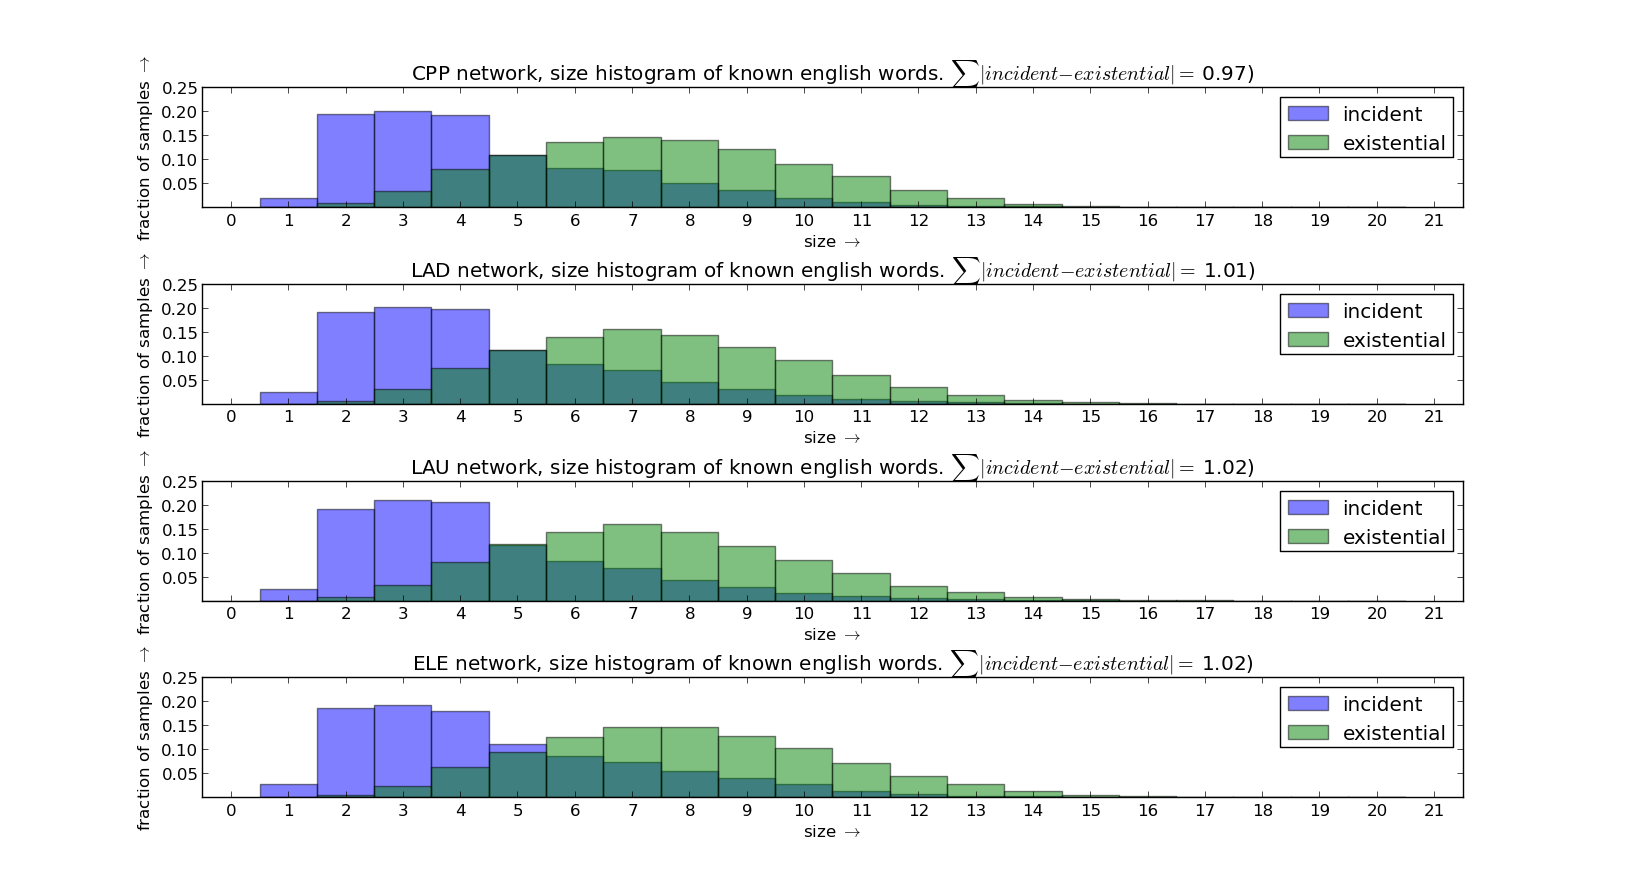
\includegraphics[width=\textwidth]{figs/kw}
    \caption{Size of words that are known in English. Crossing of incident and existential sizes is around 5 (Figure~\ref{fig:kwnsw} shows a shift to length 6-7 when consider only non stopwords). Words with three letters have maximum incidence, while most words have 7 letters. See subsection~\ref{subsec:sii} for discussion and directions.}
    \label{fig:kw}
\end{figure*}


\begin{figure*}[h!]
    \centering
    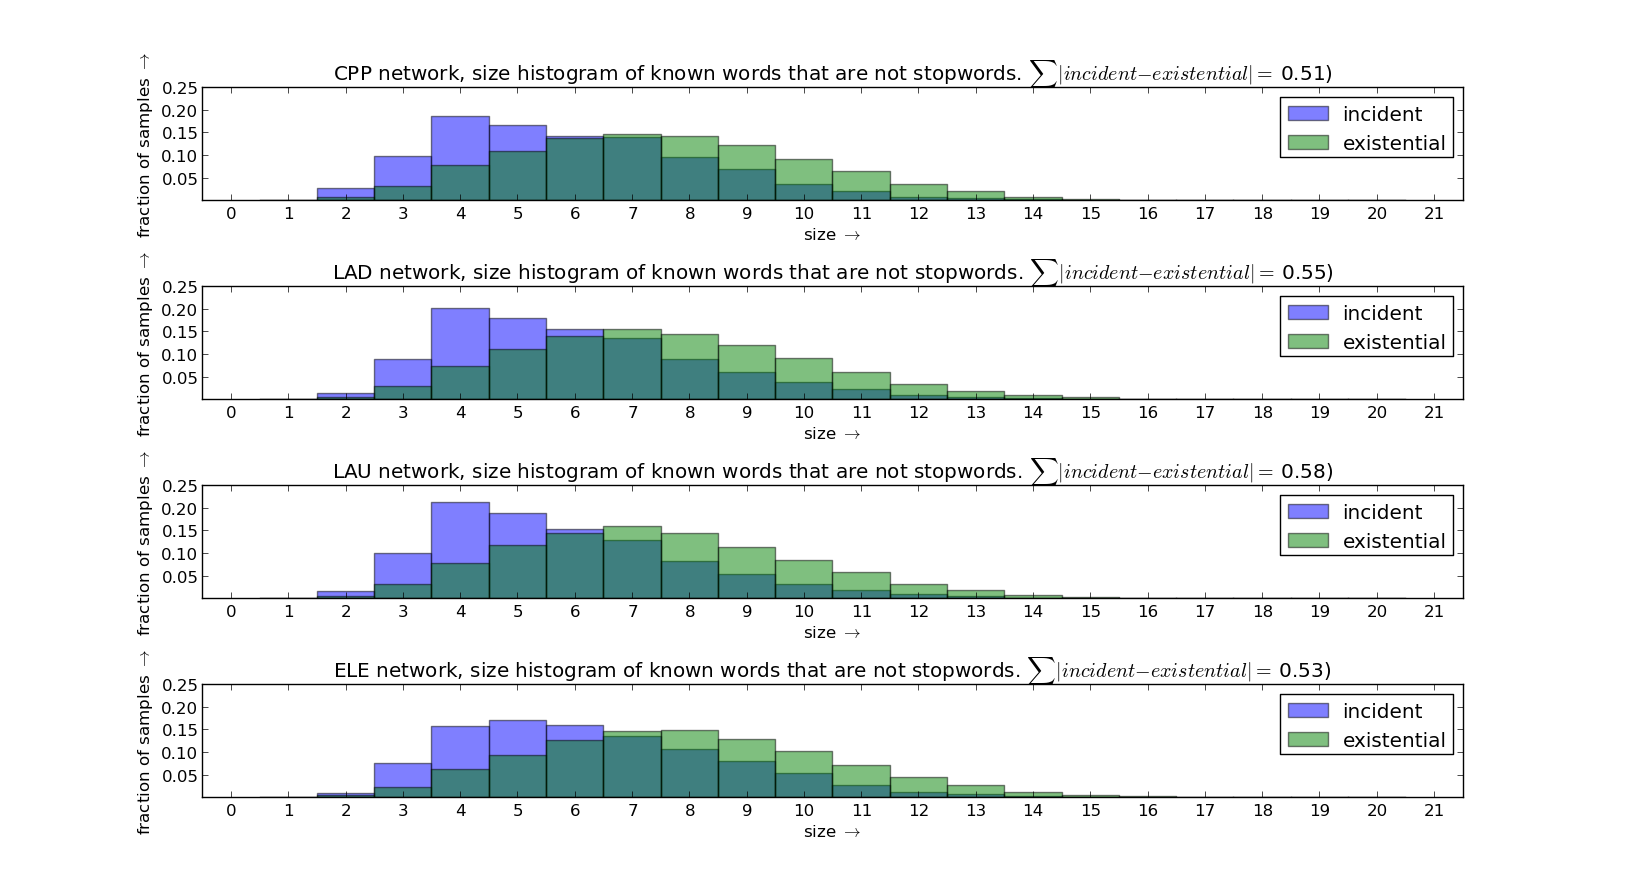
\includegraphics[width=\textwidth]{figs/kwnsw}
    \caption{Size of words that are known in English and are not stopwords. Crossing of incident and existential sizes is around 6-7 (figure~\ref{fig:kw} shows a shift to length 5 when considered stopwords). In this case, words with 4 letters have maximum incidence, while most words still have 7 letters. Exception for ELE, which exhibits maximum incidence of words with 5 letters and most words having 8 letters, which might be associated with ELE network typology discussed in tables~\ref{tab:tokens} and~\label{tab:caracteres}. See subsection~\ref{subsec:sii} for discussion and directions.}
    \label{fig:kwnsw}
\end{figure*}

\begin{figure*}[h!]
    \centering
    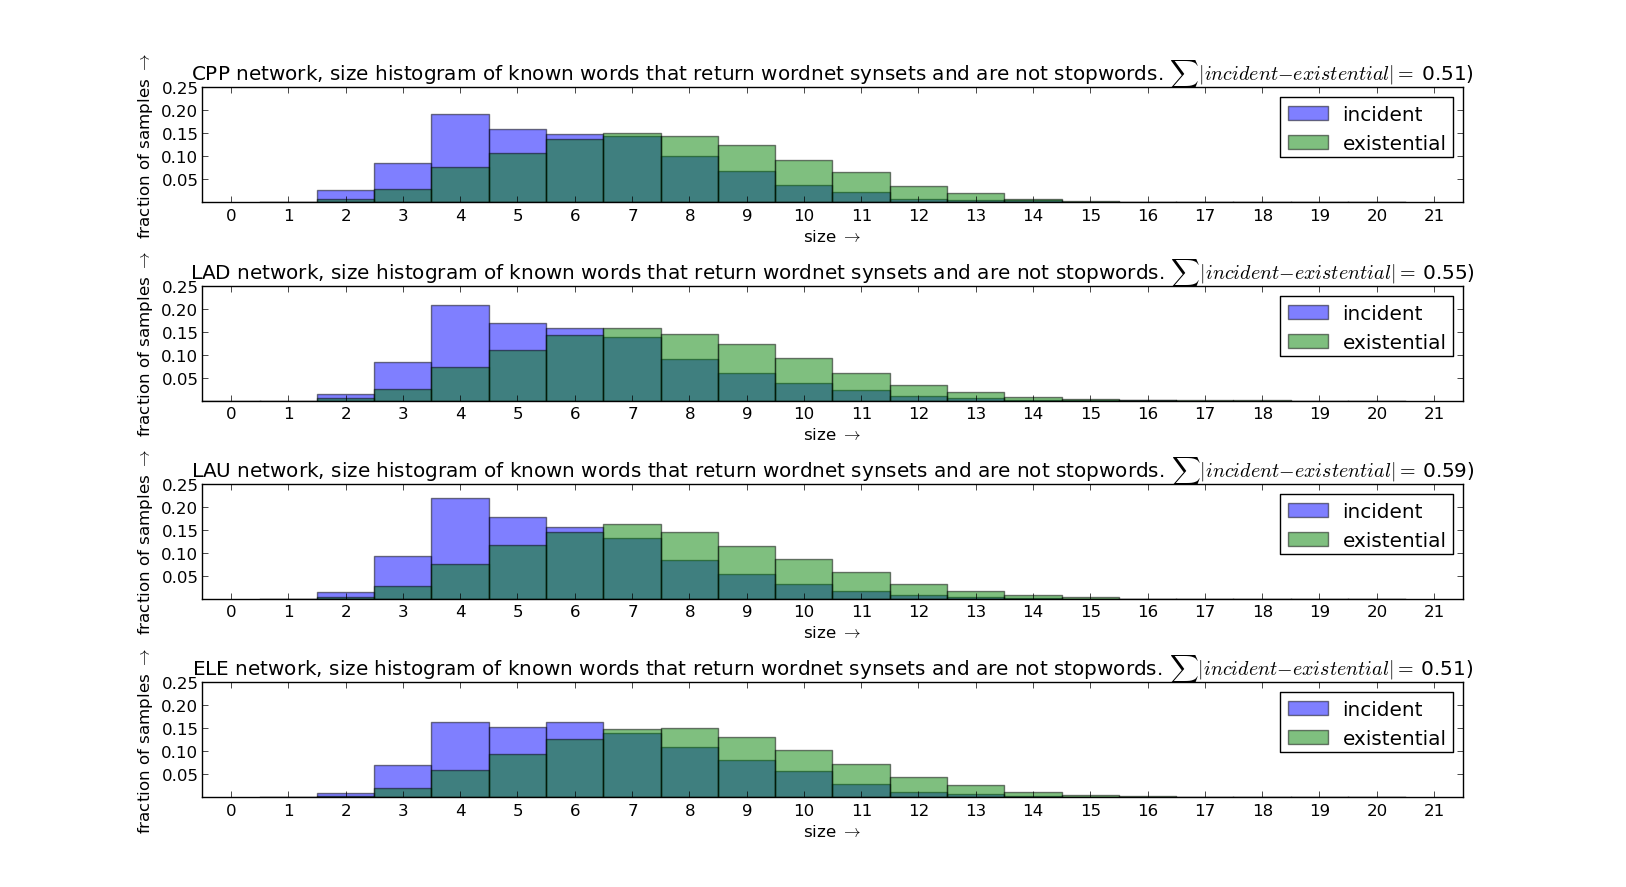
\includegraphics[width=\textwidth]{figs/kwssnsw}
    \caption{Size of words that are known, are not stopwords and have synsets. Resembles figure~\ref{fig:kwnsw}. Stopword sizes histogram are in figure~\ref{fig:sw}. Differences suggests $\approx 0.5$ might be constant. LAD and LAU exquisite vocabulary (GNU/Linux, programming, sound/signal processing, music) might be responsible for higher difference of distributions. See subsection~\ref{subsec:sii} for discussion and directions. See subsection~\ref{subsec:sii} for discussion and directions.}
    \label{fig:kwssnsw}
\end{figure*}


\begin{figure*}[h!]
    \centering
    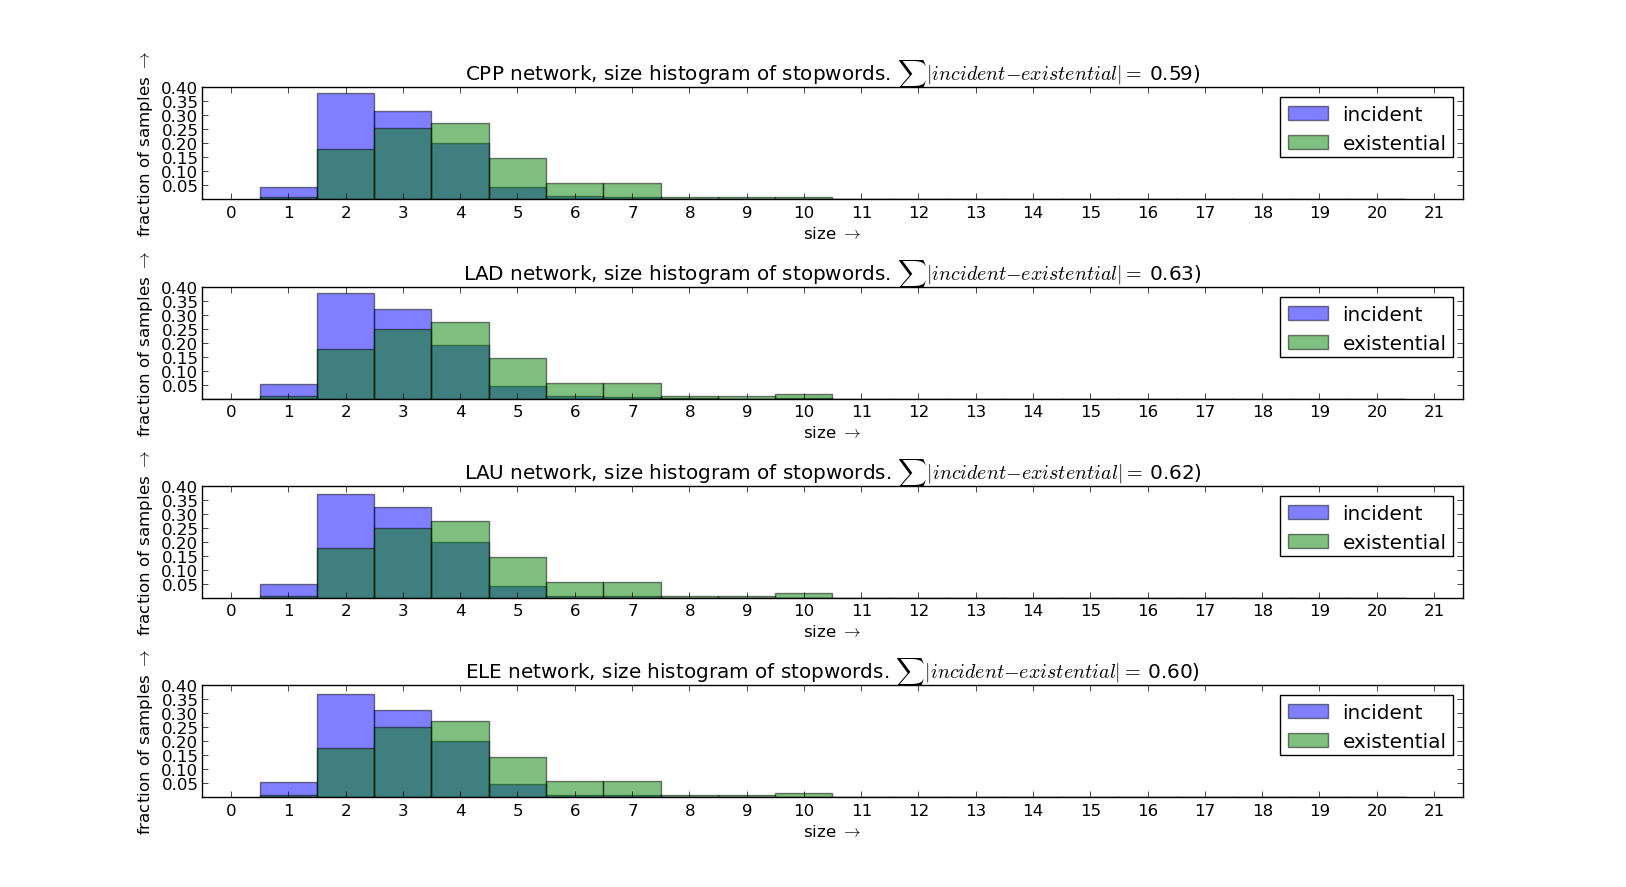
\includegraphics[width=\textwidth]{figs/sw}
    \caption{Size histogram of stopwords. Stopwords with two letters are the most frequent, while most of them have four letters. Differences in distribution seem stable around $\approx 0.6$. See subsection~\ref{subsec:sii} for discussion and directions.}
    \label{fig:sw}
\end{figure*}



\begin{figure*}[h!]
    \centering
    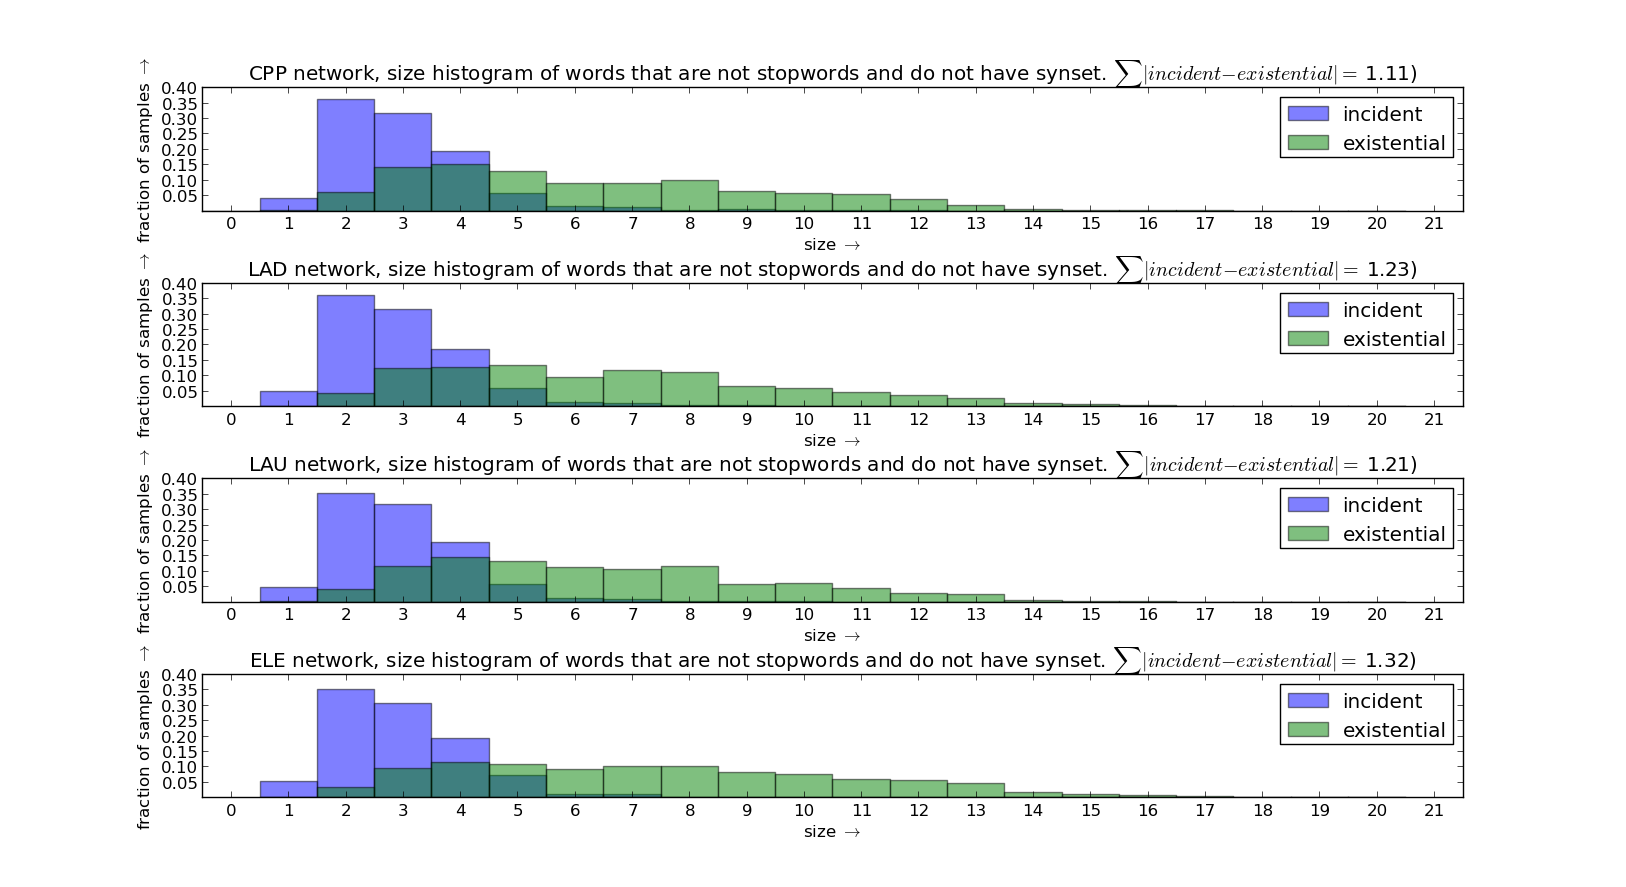
\includegraphics[width=\textwidth]{figs/nssnsw}
    \caption{Size histogram of known English words that are not stopwords and do not return synsets. Differences in distribution suggests less stable behavior, with high incidence of few words high number of existing words with many letters. Observe difference $\geq 1$, as observed only with all known words, but even higher. See subsection~\ref{subsec:sii} for discussion and directions.}
    \label{fig:nssnsw}
\end{figure*}



 
%\nocite{*}
%\nocite{*}
\bibliography{supportingInformation}% Produces the bibliography via BibTeX.
\end{document}
%
% ****** End of file aipsamp.tex ******


